\documentclass[aspectratio=169,xcolor=dvipsnames]{beamer}

% Modern colorful theme
\usetheme{Madrid}
\usecolortheme{seahorse}

% Custom colors from original thesis
\definecolor{cwAlert}{RGB}{220,50,50}
\definecolor{cwFlow}{RGB}{50,120,220}
\definecolor{cwDecoy}{RGB}{120,180,50}
\definecolor{cwBorder}{RGB}{80,80,80}
\definecolor{ImperialBlue}{RGB}{0,62,116}
\definecolor{ImperialNavy}{RGB}{0,33,71}
\definecolor{ImperialLightBlue}{RGB}{155,203,235}

% Set theme colors
\setbeamercolor{structure}{fg=ImperialBlue}
\setbeamercolor{palette primary}{bg=ImperialNavy,fg=white}
\setbeamercolor{palette secondary}{bg=ImperialBlue,fg=white}
\setbeamercolor{palette tertiary}{bg=ImperialLightBlue,fg=ImperialNavy}
\setbeamercolor{frametitle}{bg=ImperialBlue,fg=white}
\setbeamercolor{title}{fg=ImperialNavy}

% Packages
\usepackage{tikz}
\usepackage{amsmath}
\usepackage{amssymb}
\usepackage{booktabs}
\usepackage{adjustbox}
\usepackage{xcolor}
\usepackage{colortbl}
\usepackage{pgfplots}
\pgfplotsset{compat=1.18}
\usetikzlibrary{shapes,arrows,positioning,shadows,patterns}
\usetikzlibrary{shapes,arrows,positioning,shadows,patterns}
\usetikzlibrary{arrows.meta} 

% Title information
\title[Adaptive Cyber Defense with AI]{\textbf{Adaptive Resource Placement for Cyber Defense}}
\subtitle{\textbf{Better Protection Through Multi-Agent Reinforcement Learning}}
%89\%
\author[M. Akanmode]{Miracle Akanmode}
\institute[Imperial College London]{
    Department of Computing\\
    Imperial College London\\
    \vspace{0.2cm}
    Supervisor: Kelly Zhang
}
\date{September 2025}

\begin{document}

%----------------------------------------------------------------------
% TITLE SLIDE
%----------------------------------------------------------------------
\begin{frame}
\vspace{0.25cm}
% Logo in top left
\begin{flushleft}

\includegraphics[height=0.7cm]{/rds/general/user/moa324/home/projects/cyberwheel/research_docs/poster/Images/ICL_Logo_Blue_RGB.pdf}
\end{flushleft}

\vspace{0.3cm}
\begin{center}
{\LARGE\textbf{\textcolor{ImperialNavy}{Adaptive Resource Placement}}}\\[0.12cm]
{\LARGE\textbf{\textcolor{ImperialNavy}{for Cyber Defense}}}\\[0.28cm]

{\large\textcolor{ImperialBlue}{Better Protection Through}}\\[0.08cm]
{\large\textcolor{ImperialBlue}{Multi-Agent Reinforcement Learning}}\\[0.4cm]
{\large\textbf{Miracle Akanmode}}\\[0.06cm]
{\normalsize Imperial-X}\\[0.07cm]
{\normalsize Imperial College London}\\[0.06cm]
\end{center}

\vfill
\begin{columns}[t]
    \column{0.5\textwidth}
    \begin{flushleft}
        {\normalsize Project Defense: September 2025}\\[0.06cm]
        {\normalsize Supervisor: Kelly Zhang}\\%[0.3cm]
    \end{flushleft}
        
    \column{0.5\textwidth}
    \begin{flushright}
        {\small\textcolor{ImperialBlue}{miracle.akanmode24@imperial.ac.uk}}
    \end{flushright}
\end{columns}
\vspace{1mm}
\end{frame}

%----------------------------------------------------------------------
% RESEARCH OVERVIEW
%----------------------------------------------------------------------
\begin{frame}{Research Overview}
\begin{columns}[c]
\column{0.6\textwidth}
\begin{itemize}
    \item \textbf{\textcolor{cwAlert}{Problem}}: Static cyber defenses fail against adaptive adversaries
    \item \textbf{\textcolor{cwFlow}{Approach}}: Multi-agent reinforcement learning for adaptive deception
    \item \textbf{\textcolor{cwDecoy}{Solution}}: PPO-based agent learning optimal honeypot placement
    \item \textbf{\textcolor{ImperialBlue}{Result}}: \textbf{89\% performance improvement} over baselines
\end{itemize}

\column{0.4\textwidth}
\begin{center}
\begin{center}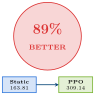
\includegraphics[width=0.95\columnwidth]{figures/fig_1.svg}\end{center}
\end{center}
\end{columns}
\end{frame}

% ---------------------------------------------------------------------
% Quotes
% ---------------------------------------------------------------------
\begin{frame}{Ancient War Strategy Quotes}
\begin{block}{Sun Tzu Quotes}
\small
\begin{itemize}
  \item ``All warfare is based on deception.''
  \item ``He will win who knows when to fight and when not to fight.''
  \item ``The greatest victory is that which requires no battle.'' --- Sun Tzu, The Art of War.
\end{itemize}
\end{block}

\vspace{6pt}
\small These quotes support our approach: creating uncertainty and choosing when to act are central to the defense agent's strategy.
\end{frame}


%----------------------------------------------------------------------
% KEY TERMS & CONCEPTS  
%----------------------------------------------------------------------

\begin{frame}{Key Terms \& Concepts}
\small
\begin{columns}[t]
  \column{0.48\textwidth}
  \begin{description}[leftmargin=!,labelwidth=2.8cm]
    \item[\textbf{Reinforcement Learning}] Learning by trial and reward feedback.
    \item[\textbf{Agent}] The automated decision-maker (here: Blue agent).
    \item[\textbf{Environment}] The simulated network in which agents act.
    \item[\textbf{Policy}] Mapping from what the agent sees to actions.
    \item[\textbf{Reward}] Numeric signal that guides learning (good/bad).
  \end{description}

  \column{0.48\textwidth}
  \begin{description}[leftmargin=!,labelwidth=2.8cm]
    \item[\textbf{PPO}] A stable policy-optimisation algorithm used here.
    \item[\textbf{Action}] What the agent does (deploy/remove/wait).
    \item[\textbf{Observation / State}] What the agent perceives about the network.
    \item[\textbf{Honeypot / Decoy}] Fake asset used to lure and study attackers.
    \item[\textbf{Red / Blue Team}] Red = attacker (fixed); Blue = defender (learning).
  \end{description}
\end{columns}

\vspace{4pt}
\small Additional: MITRE ATT\&CK = standardised attacker techniques; "deception" = deliberate uncertainty creation to mislead attackers.
\end{frame}

%----------------------------------------------------------------------
% THE PROBLEM
%----------------------------------------------------------------------
\begin{frame}{The Cybersecurity Challenge}
\begin{columns}[c]
\column{0.5\textwidth}
\textbf{\textcolor{cwAlert}{Critical Challenges:}}
\begin{itemize}
    \item \textbf{Alert Fatigue}: 4,000+ daily alerts, 67\% ignored
    \item \textbf{Asymmetric Warfare}: Attackers need one success
    \item \textbf{Static Defenses}: Predictable patterns exploited
    \item \textbf{Base-Rate Fallacy}: Real threats missed
\end{itemize}

\column{0.5\textwidth}
\begin{center}
\begin{center}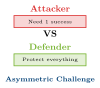
\includegraphics[width=0.95\columnwidth]{figures/fig_2.svg}\end{center}
\end{center}
\end{columns}

\vspace{0.5cm}
\begin{alertblock}{Our Solution}
\textbf{Adaptive AI-driven deception} that creates uncertainty for attackers through learned strategic honeypot placement
\end{alertblock}
\end{frame}


%----------------------------------------------------------------------
% DEFENSE EVOLUTION - EXACT TIKZ FROM ORIGINAL
%----------------------------------------------------------------------
\begin{frame}{Evolution of Cyber Defense}
\begin{center}
\scalebox{0.7}{
\begin{center}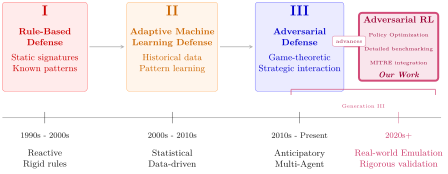
\includegraphics[width=0.95\columnwidth]{figures/fig_3.svg}\end{center}
}
\end{center}
\end{frame}


% ---------------------------------------------------------------------
% NEW SLIDE: Network diagram (schematic)
% ---------------------------------------------------------------------

\begin{frame}{Network and Agent Environment Overview}
\begin{center}
\begin{adjustbox}{max width=\columnwidth,max totalheight=0.78\textheight,center}
\begin{center}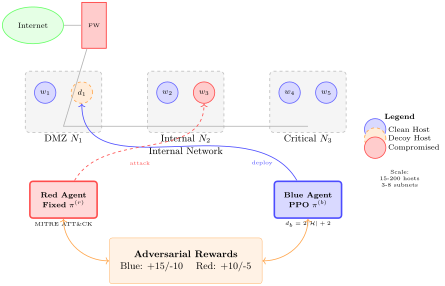
\includegraphics[width=0.95\columnwidth]{figures/fig_4.svg}\end{center}
\end{adjustbox}
\end{center}
\vspace{-2mm}
\end{frame}

%----------------------------------------------------------------------
% PPO ARCHITECTURE - EXACT TIKZ FROM ORIGINAL
%----------------------------------------------------------------------
\begin{frame}{PPO Training Architecture}
\begin{center}
\scalebox{0.8}{
\begin{center}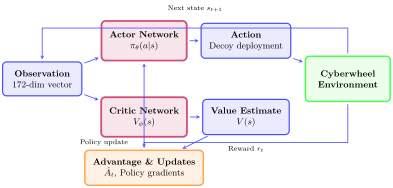
\includegraphics[width=0.95\columnwidth]{figures/fig_5.svg}\end{center}
}
\end{center}

\begin{block}{Key Features}
\begin{itemize}
\item \textbf{172-dimensional observation space}: Alert history + network state + metadata  
\item \textbf{Actor-critic framework}: Stable policy optimization with value function guidance
\item \textbf{Strategic reward feedback}: Learn optimal deception placement through experience
\end{itemize}
\end{block}
\end{frame}

% ---------------------------------------------------------------------
% NEW SLIDE: RL Foundations (PPO math)
% ---------------------------------------------------------------------
\begin{frame}{RL Foundations (PPO — concise)}
\scriptsize
\begin{align*}
  &\pi_\theta(a|s)\quad\text{(actor / policy)}\\
  &V_\phi(s)\quad\text{(critic / value)}\\[4pt]
  &r_t(\theta)=\frac{\pi_\theta(a_t|s_t)}{\pi_{\theta_{\text{old}}}(a_t|s_t)}\\[2pt]
  &L^{\mathrm{CLIP}}(\theta)=\mathbb{E}_t\Big[\min\big(r_t(\theta)\,\hat A_t,\ \mathrm{clip}(r_t(\theta),1-\epsilon,1+\epsilon)\,\hat A_t\big)\Big]\\[6pt]
  &L(\theta,\phi)= -L^{\mathrm{CLIP}}(\theta) \;+\; c_1\,(V_\phi(s_t)-R_t)^2 \;-\; c_2\,\mathcal H(\pi_\theta)\\[6pt]
  &\text{GAE (compact): }\quad \hat A_t=\sum_{l=0}^{k-1}(\gamma\lambda)^l\delta_{t+l},\qquad 
  \delta_t=r_t+\gamma V_\phi(s_{t+1})-V_\phi(s_t)
\end{align*}

\vspace{4pt}
\small Notes: clipping stabilises policy updates; value loss (c1) and entropy regulariser (c2) improve convergence.
\end{frame}

%----------------------------------------------------------------------
% EXPERIMENTAL RESULTS
%----------------------------------------------------------------------
\begin{frame}{Key Results: 89\% Performance Improvement}
\begin{columns}[c]
\column{0.45\textwidth}
\textbf{\textcolor{ImperialBlue}{Algorithm Performance:}}

\centering
\begin{tabular}{|l|c|}
\hline
\rowcolor{ImperialLightBlue}
\textbf{Algorithm} & \textbf{Reward} \\
\hline
\rowcolor{green!20}
\textbf{PPO (Ours)} & \textbf{309.14} \\
Static Baseline & 163.81 \\
Rule Baseline & 79.16 \\
Inactive & -1.61 \\
\hline
\end{tabular}


\column{0.55\textwidth}
\textbf{\textcolor{cwAlert}{Security Effectiveness:}}
\begin{itemize}
    \item \textbf{\textcolor{cwAlert}{89\% improvement}} over static baseline
    \item \textbf{73.2\% deception success} rate (vs 45.1\% static)
    \item \textbf{82.4\% asset protection} rate (vs 61.7\% static)
    \item \textbf{2.3 timestep} detection latency (vs 4.1 static)
    \item \textbf{92.3\% correlation} with MITRE ATT\&CK patterns
    \item \textbf{84.8\% defense success} against real attacks
\end{itemize}
\end{columns}

\vspace{0.3cm}
\begin{exampleblock}{Statistical Validation}
\textbf{ANOVA p < 0.001}, Cohen's d > 0.8, 95\% confidence intervals, 5-seed validation
\end{exampleblock}
\end{frame}

%----------------------------------------------------------------------
% STRATEGIC BEHAVIORS
%----------------------------------------------------------------------
\begin{frame}{Learned Strategic Behaviors}
\begin{columns}[c]
\column{0.6\textwidth}
\textbf{\textcolor{ImperialBlue}{Emergent Intelligence:}}
\begin{itemize}
    \item \textbf{Balanced Strategy}: 20.4\% deploy, 19.2\% remove, 60.4\% wait
    \item \textbf{Learned Restraint}: Avoids over-deployment traps
    \item \textbf{Superior Consistency}: $\sigma = 37.37$ vs baseline variance
    \item \textbf{Adaptive Timing}: Strategic waiting periods
\end{itemize}

\textbf{\textcolor{cwDecoy}{Strategic Insights:}}
\begin{itemize}
    \item Agent learns \textbf{when NOT to act} (patience)
    \item Balances resource costs vs security benefits
    \item Adapts to attacker patterns without explicit programming
\end{itemize}

\column{0.4\textwidth}
\begin{center}
% Clean, self-contained pie chart. Wait leader forced straight down.
\begin{center}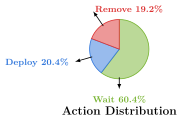
\includegraphics[width=0.95\columnwidth]{figures/fig_6.svg}\end{center}
\end{center}
\end{columns}
\end{frame}

%----------------------------------------------------------------------
% SCALABILITY ANALYSIS
%----------------------------------------------------------------------
\begin{frame}{Scalability Analysis}
\begin{columns}[c]
\column{0.5\textwidth}
\textbf{\textcolor{ImperialBlue}{Network Size Performance:}}

\begin{center}
\begin{tabular}{|l|c|c|}
\hline
\rowcolor{ImperialLightBlue}
\textbf{Hosts} & \textbf{Reward} & \textbf{Time} \\
\hline
15 & 309.14 & 2.5h \\
50 & 325.42 & 6.2h \\
200 & 298.17 & 18.4h \\
\hline
\end{tabular}
\end{center}

\textbf{\textcolor{cwDecoy}{Scalability Properties:}}
\begin{itemize}
    \item \textbf{Consistent Performance}: 298-325 reward range
    \item \textbf{Sub-quadratic scaling}: O(n log n) complexity
    \item \textbf{Linear memory usage}: Practical for enterprise
    \item \textbf{Strategic consistency}: Behaviors stable across scales
\end{itemize}

\column{0.5\textwidth}
%\begin{center}
\textbf{Performance vs Network Size}

%\begin{center}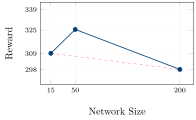
\includegraphics[width=0.95\columnwidth]{figures/fig_7.svg}\end{center}
\end{center}

\textbf{\textcolor{cwAlert}{Enterprise Ready:}} Validated up to 200 hosts with maintained effectiveness
\end{columns}
\end{frame}

%----------------------------------------------------------------------
% REAL-WORLD VALIDATION
%----------------------------------------------------------------------
\begin{frame}{Real-World Validation}
\begin{columns}[c]
\column{0.5\textwidth}
\textbf{\textcolor{ImperialBlue}{MITRE ATT\&CK Integration:}}
\begin{itemize}
    \item \textbf{295 attack techniques} implemented
    \item \textbf{92.3\% behavioral correlation} with real patterns
    \item \textbf{Complete kill chain} coverage (4 phases)
    \item \textbf{Atomic Red Team} validation
\end{itemize}

\textbf{\textcolor{cwDecoy}{Attack Defense Success:}}
\begin{itemize}
    \item \textbf{84.8\% success rate} against real attack commands
    \item \textbf{Early disruption}: 2.3 timestep detection
    \item \textbf{Proactive defense}: Uncertainty creation vs reactive response
\end{itemize}

\column{0.5\textwidth}
\begin{center}
\begin{center}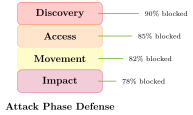
\includegraphics[width=0.95\columnwidth]{figures/fig_8.svg}\end{center}
\end{center}
\end{columns}

\vspace{0.3cm}
\begin{alertblock}{Practical Deployment Ready}
\textbf{Enterprise-scale validation} with realistic attack patterns and \textbf{consistent cross-scale performance}
\end{alertblock}
\end{frame}

%----------------------------------------------------------------------
% METHODOLOGY
%----------------------------------------------------------------------
\begin{frame}{Research Methodology}
\begin{columns}[c]
\column{0.5\textwidth}
\textbf{\textcolor{ImperialBlue}{Experimental Framework:}}
\begin{itemize}
    \item \textbf{Multi-Agent Setup}: Learning blue vs fixed red (295 techniques)
    \item \textbf{Networks}: 15-200 hosts, realistic enterprise topologies
    \item \textbf{Training}: 10M timesteps, 5 random seeds
    \item \textbf{Baselines}: Static, Rule-based, Random, Inactive
\end{itemize}

\textbf{\textcolor{cwDecoy}{Statistical Rigor:}}
\begin{itemize}
    \item \textbf{ANOVA}: p < 0.001 significance
    \item \textbf{Effect Size}: Cohen's d > 0.8 (large)
    \item \textbf{Confidence}: 95\% intervals
    \item \textbf{Reproducibility}: 5-seed validation
\end{itemize}

\column{0.5\textwidth}
\textbf{\textcolor{cwAlert}{Novel Contributions:}}
\begin{enumerate}
    \item \textbf{First systematic PPO validation} for cyber deception
    \item \textbf{Real-world MITRE integration} with 92.3\% fidelity
    \item \textbf{Scalability characterization} across enterprise networks
    \item \textbf{Strategic behavior analysis} revealing emergent intelligence
    \item \textbf{Reproducible methodology} with open protocols
\end{enumerate}

\textbf{\textcolor{ImperialBlue}{Research Questions Answered:}}
\begin{itemize}
    \item PPO effectively learns adaptive strategies
    \item 89\% improvement over traditional baselines
    \item Strategic behaviors emerge and scale robustly
\end{itemize}
\end{columns}
\end{frame}

%----------------------------------------------------------------------
% FUTURE WORK
%----------------------------------------------------------------------
\begin{frame}{Future Directions \& Impact}
\scriptsize
\setlength{\parskip}{0pt}
\setlength{\topsep}{0pt}
\begin{columns}[t]
  % use a wider left column so content fills the available space
  \column{0.62\textwidth}
  \textbf{Research Extensions:}
  \vspace{2pt}
  {\setlength{\parskip}{0pt}%
   \begin{itemize}
     \item Real-world deployment in operational environments
     \item Adversarial co-evolution with learning attackers (self-play)
     \item Multi-defender coordination across distributed networks
     \item Integration with existing security infrastructure (SIEM, EDR)
     \item Explainable AI for analyst understanding and trust
   \end{itemize}
  }

  \vspace{4pt}
  \textbf{Technical Advances:}
  \vspace{2pt}
  {\setlength{\parskip}{0pt}%
   \begin{itemize}
     \item Advanced reward shaping for complex scenarios
     \item Transfer learning across network topologies
     \item Real-time adaptation to novel attack patterns
   \end{itemize}
  }

  \column{0.38\textwidth}
  \begin{block}{Broader Impact}
  \tiny
  This work establishes reinforcement learning as a viable approach for automated cybersecurity defense with rigorous experimental validation.
  \end{block}

  \vspace{4pt}
  \begin{block}{Key Takeaways}
  \tiny
  \begin{itemize}
      \item AI successfully learns sophisticated adaptive defense strategies
      \item \textbf{89\% improvement} demonstrates clear superiority
      \item Strategic restraint emerges naturally without explicit programming
      \item Performance scales robustly to enterprise networks
      \item Real attack correlation validates deployment readiness
  \end{itemize}
  \end{block}
\end{columns}
\end{frame}




%----------------------------------------------------------------------
% CONCLUSIONS
%----------------------------------------------------------------------
\begin{frame}{Conclusions}
\begin{center}
{\Large\textbf{\textcolor{ImperialNavy}{Adaptive AI-Driven Cyber Defense Works}}}
\end{center}

\begin{columns}[c]
\column{0.33\textwidth}
\begin{block}{\textcolor{cwAlert}{Performance}}
\begin{center}
{\huge\textbf{89\%}}\\
\textbf{Improvement}\\
over static baselines
\end{center}
\end{block}

\column{0.33\textwidth}
\begin{block}{\textcolor{cwFlow}{Intelligence}}
\begin{center}
\textbf{Strategic}\\
\textbf{Behaviors}\\
emerge naturally
\end{center}
\end{block}

\column{0.33\textwidth}
\begin{block}{\textcolor{cwDecoy}{Scale}}
\begin{center}
\textbf{Enterprise}\\
\textbf{Ready}\\
15-200 hosts validated
\end{center}
\end{block}
\end{columns}

\vspace{0.5cm}

\begin{alertblock}{Research Impact}
\textbf{First rigorous validation} of reinforcement learning for cybersecurity deception with \textbf{real-world attack correlation} and \textbf{enterprise-scale deployment readiness}
\end{alertblock}

\vspace{0.3cm}
\begin{center}
\textcolor{ImperialBlue}{\textbf{Questions?}}\\
\textcolor{ImperialBlue}{miracle.akanmode24@imperial.ac.uk}
\end{center}
\end{frame}

\end{document}